\section{Simulación }

En esta parte de la memoria presentamos el funcionamiento de la simulación, basada en un método de Monte-Carlo, tal y como especificamos a continuación. Hay que tener en cuenta que queremos simular las interacciones de $^{11}\text{Li}(d,t)^{10}\text{Li}$ donde en núcleo incidente es el $^{11}\text{Li}$. Nos queremos centrar en esta interacción, por lo que no vamos a considerar otras interacciones.

\begin{enumerate}

    \item  Debido a la naturaleza de estado no ligado del $^{10}$Li este aparece como una resonancia, por lo que manera intrínseca la energía de excitación del núcleo sigue una distribución de Breit-Wigner, que tendremos que tener en cuenta. Así pues, con cada interacción generaremos a partir de la energía resonante media $E^*$ y la anchura de la resonancia $\Gamma(E^*)$ un valor aleatorio que siga dicha distribución, como se puede ver en \cref{Fig:04-Ex0} y \cref{Fig:04-Ex2}.
    

    \begin{minipage}{0.45\linewidth} \centering
        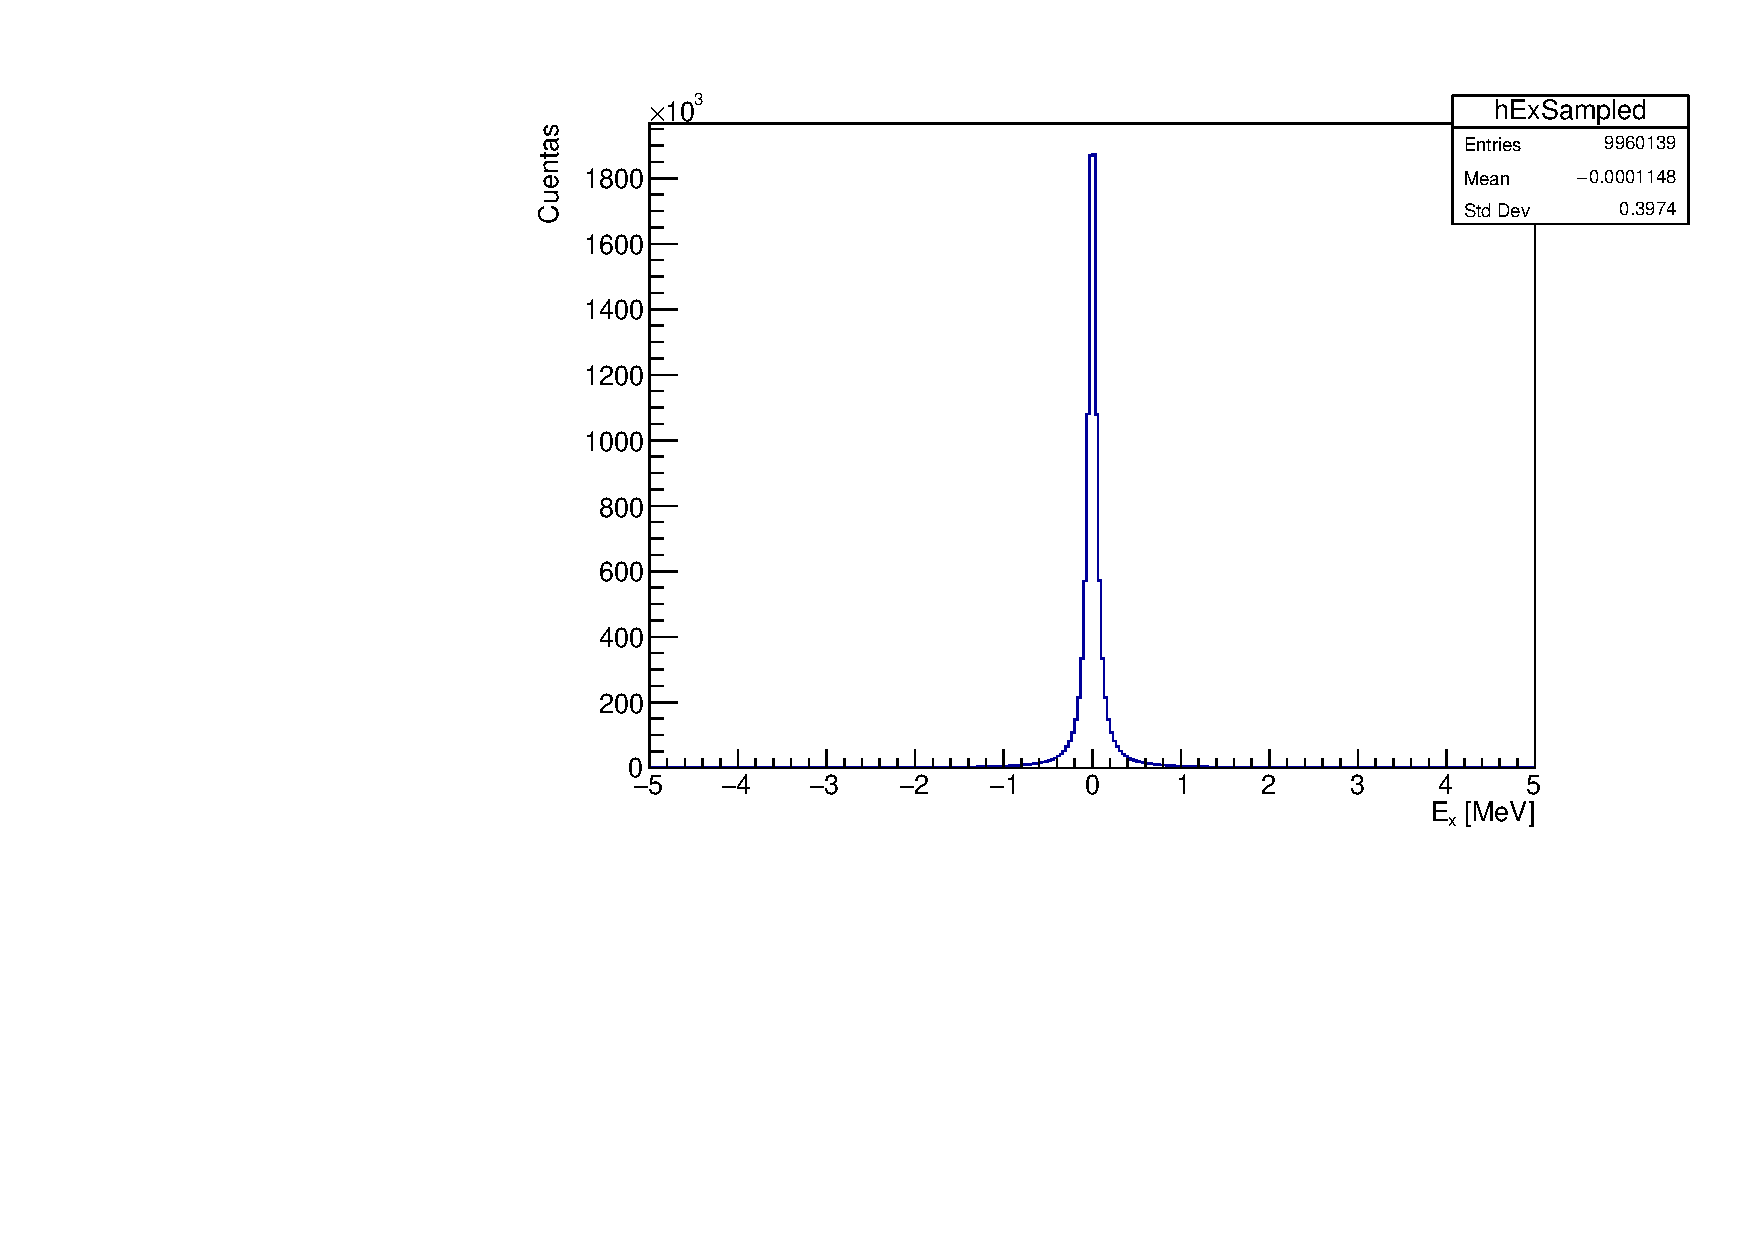
\includegraphics[width=1\linewidth]{Imagenes/ExSampled_Ex0.00_incIdx0.pdf} 
        \captionof{figure}{Distribución de las energías de excitación sampleadas $E^*=0.0$ MeV y $\Gamma=0.1$ MeV.}

        \label{Fig:04-Ex0}
    \end{minipage} \hfill
    \begin{minipage}{0.45\linewidth}
        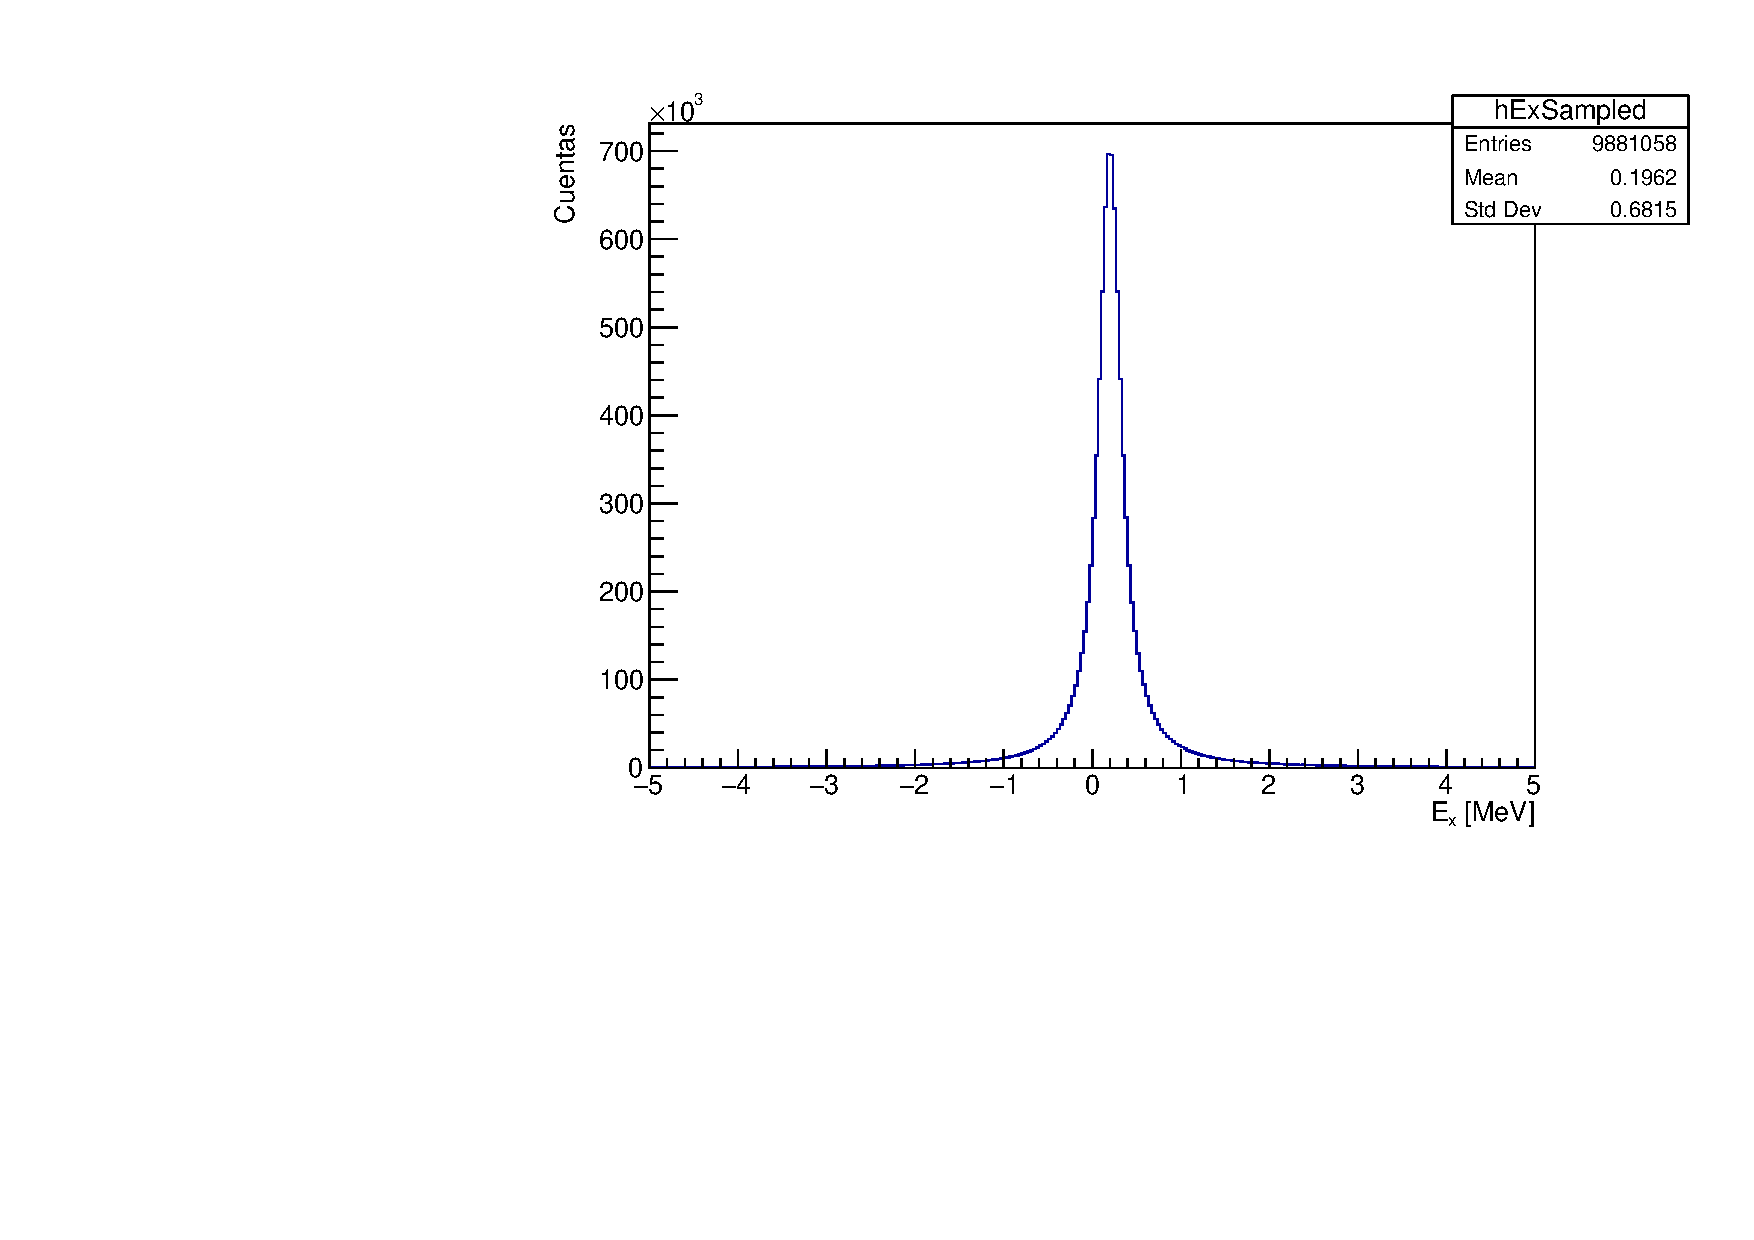
\includegraphics[width=1\linewidth]{Imagenes/ExSampled_Ex0.20_incIdx0.pdf} 
        \captionof{figure}{Distribución de las energías de excitación sampleadas $E^*=0.2$ MeV y $\Gamma=0.3$ MeV.}

        \label{Fig:04-Ex2}
    \end{minipage}
    
    

    \item  Suponemos que el haz incidente tiene una energía de $7.5$ MeV/A, que interacciona en un punto aleatorio a lo largo de la dirección del haz con una dirección $\hnx$. El punto de interacción se elige de forma aleatoria, con una distribución uniforme a lo largo del eje x a lo largo de la dimensión de la cámara de derivada, mientras que en los ejes z e y se eligen a través de una distribución gaussiana centrada en el centro de la cámara de deriva con $\sigma= 5$ mm, tal y como 
    mostramos en \cref{Fig:04-Vertex}.


    \begin{center}
        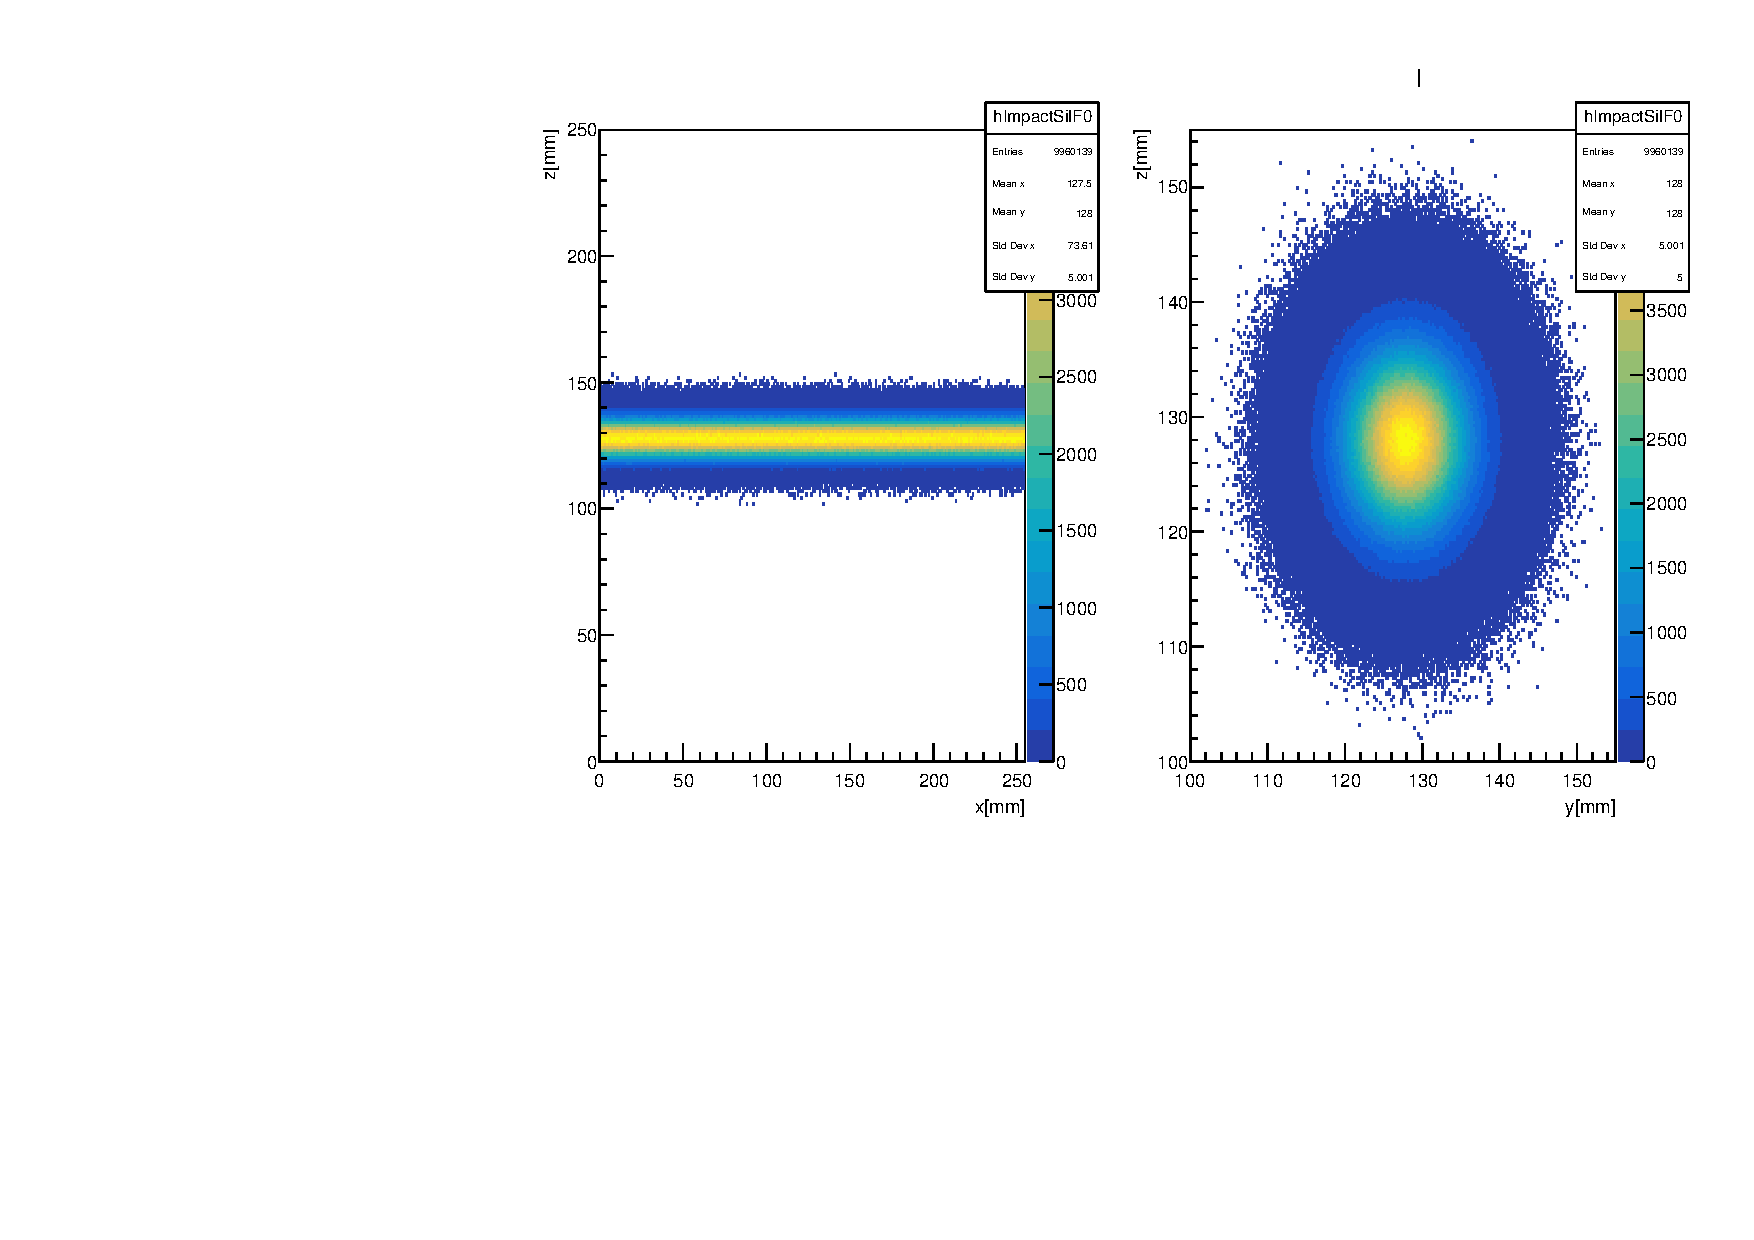
\includegraphics[width=0.65\linewidth]{Imagenes/Vertex_Ex0.00_incIdx0.pdf}
        \captionof{figure}{Distribución de las colisiones en las 4 layers. En este caso la energía de excitación del $^{10}$Li es $0$ MeV.}
        \label{Fig:04-Vertex}
    \end{center}
    
    

    \item Lo siguiente es considerar es la cinemática. Una vez elegido la $E_{ex}$ y el punto de interacción, lo que tenemos que hacer es calcular la energía cinética y ángulo en el sistema laboratorio del tritio. Será fundamental considerar la energía cinética del $^{11}$Li, que al haber recorrido una distancia $d$ aleatoria su energía se habrá reducido, por lo que tendremos que aplicar la ecuación de Bethe y el Straggling para obtener la verdadera energía cinética de $^{11}$Li en el punto de itneracción. Para conocer la dirección de salida del tritio y su energía tendremos que generar un valor aleatorio de la distribución del ángulo en el centro de masas $\phi_{CM}$ que por definición será igual que $\phi_{lab}$, y vendrá dado por una distibución uniforme entre $0$ y $2\pi$. El valor de $\theta_{CM}$ por otro lado vendrá dado por la distribución de la sección eficaz diferencial de la reacción, que podemos ver en la \cref{Fig:04-seccion_eficaz}.
    

    \begin{center}
        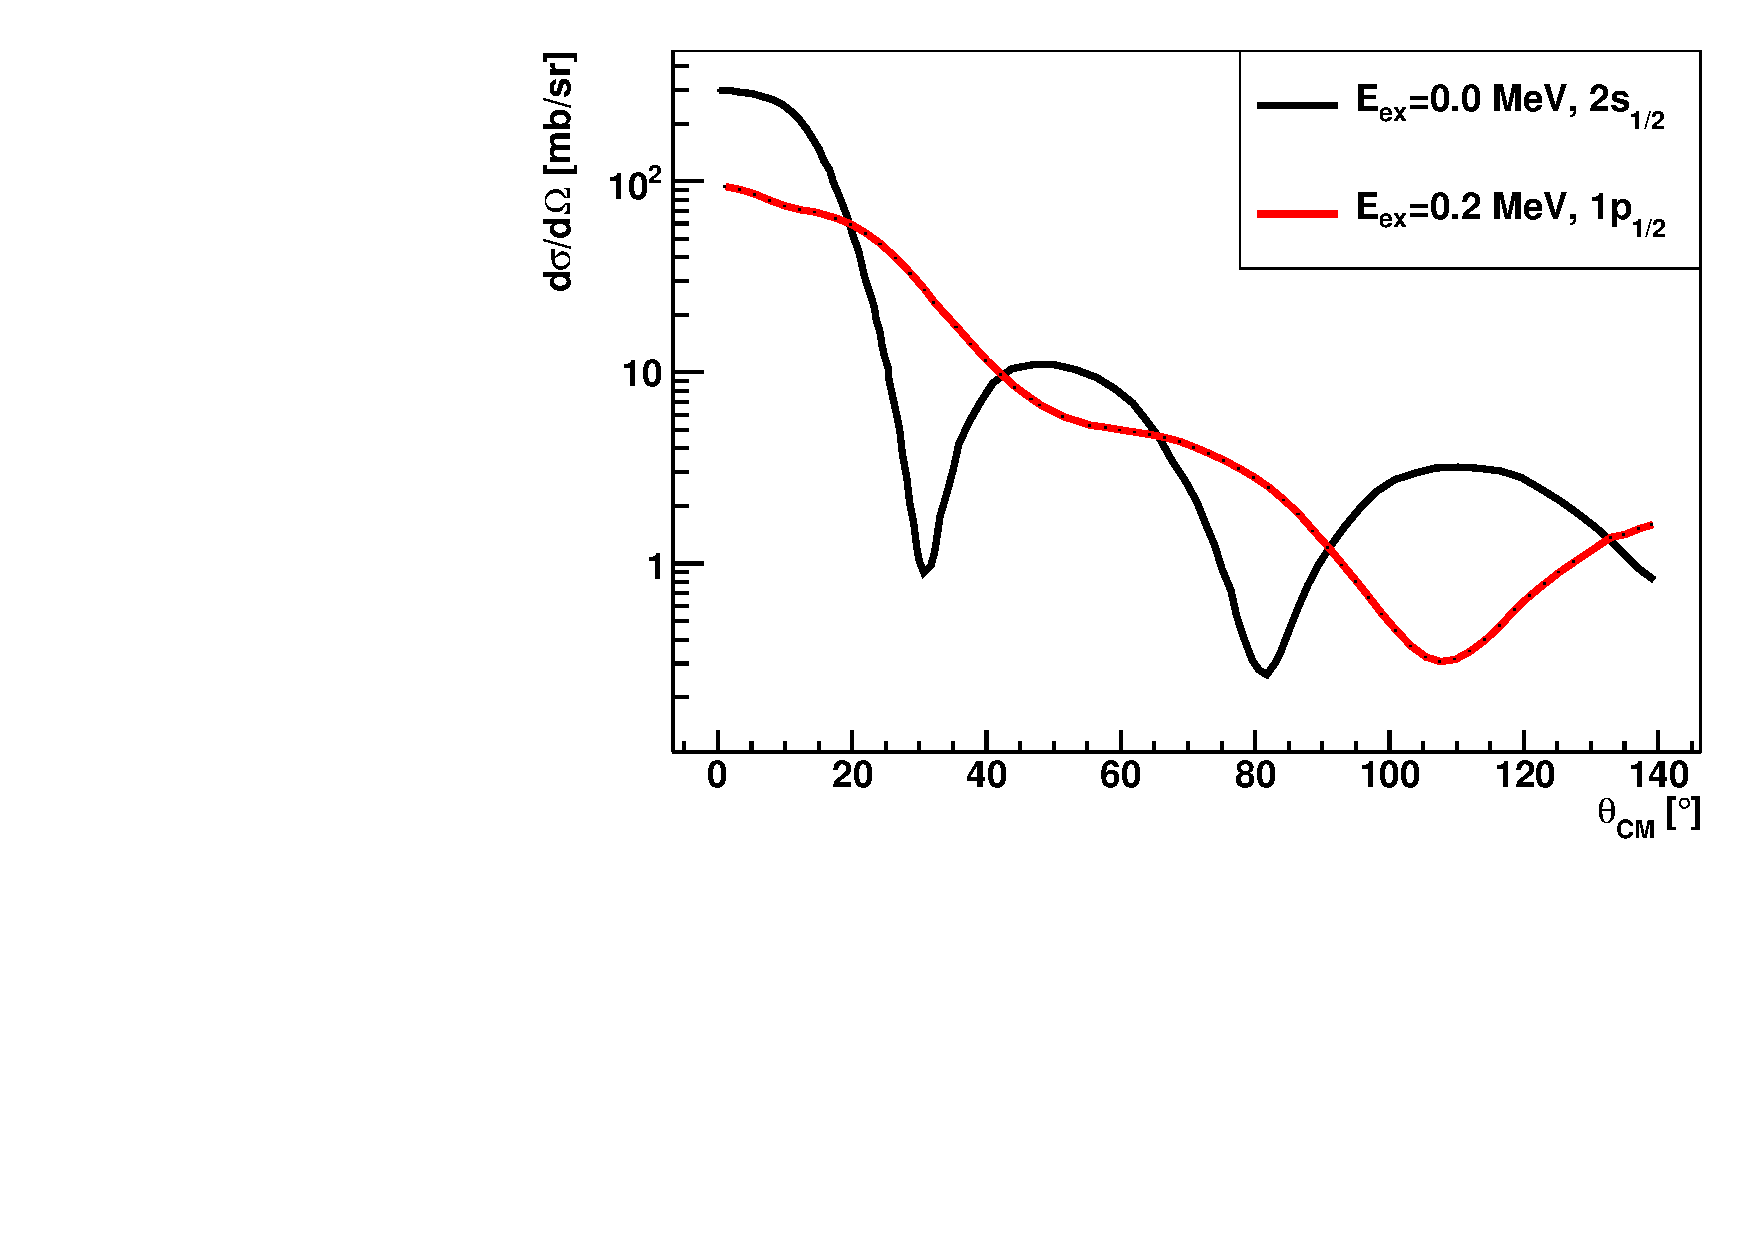
\includegraphics[width=0.7\linewidth]{Imagenes/Seccion_Eficaz.pdf}
        \captionof{figure}{Sección eficaz teórica que usaremos para ambas excitaciones.}
        \label{Fig:04-seccion_eficaz}
    \end{center}
    
    A través de las ecuaciones del apartado \ref{Subsec:03-cinematica} podremos obtener $T_{lab}$ y la dirección del tritio en el sistema laboratorio. Podemos ver en la \cref{Fig:04-kinSampled0} y \cref{Fig:04-kinSampled2} el valor de la energía cinética del tritio y el ángulo de salida, en un gráfico denominada cinemática de la reacción, en función de la energía de excitación.
    
    \begin{minipage}{0.45\linewidth} \centering
        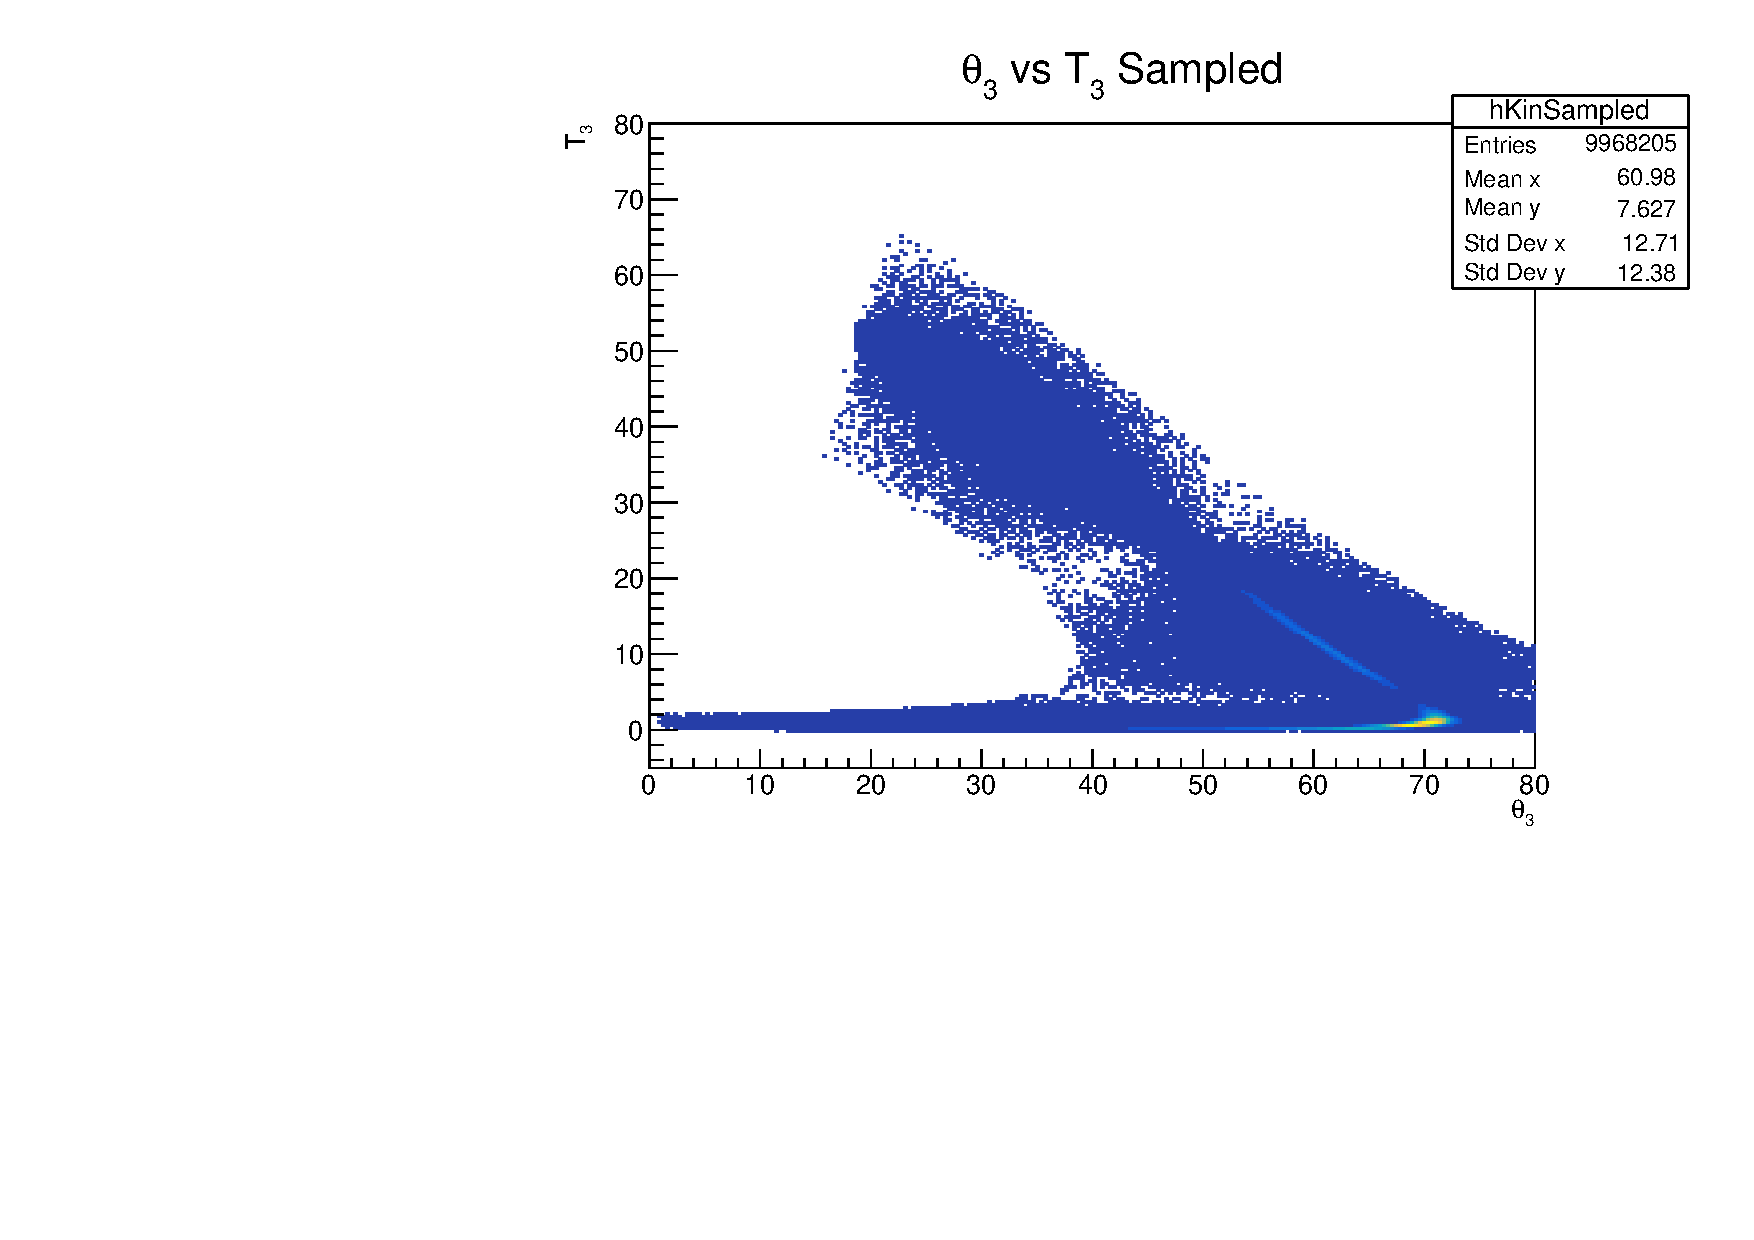
\includegraphics[width=1\linewidth]{Imagenes/KinSampled_Ex0.00_incIdx0.pdf} 
        \captionof{figure}{Cinemática sampleada para $E^*=0.0$ MeV.}

        \label{Fig:04-kinSampled0}
    \end{minipage} \hfill
    \begin{minipage}{0.45\linewidth}
        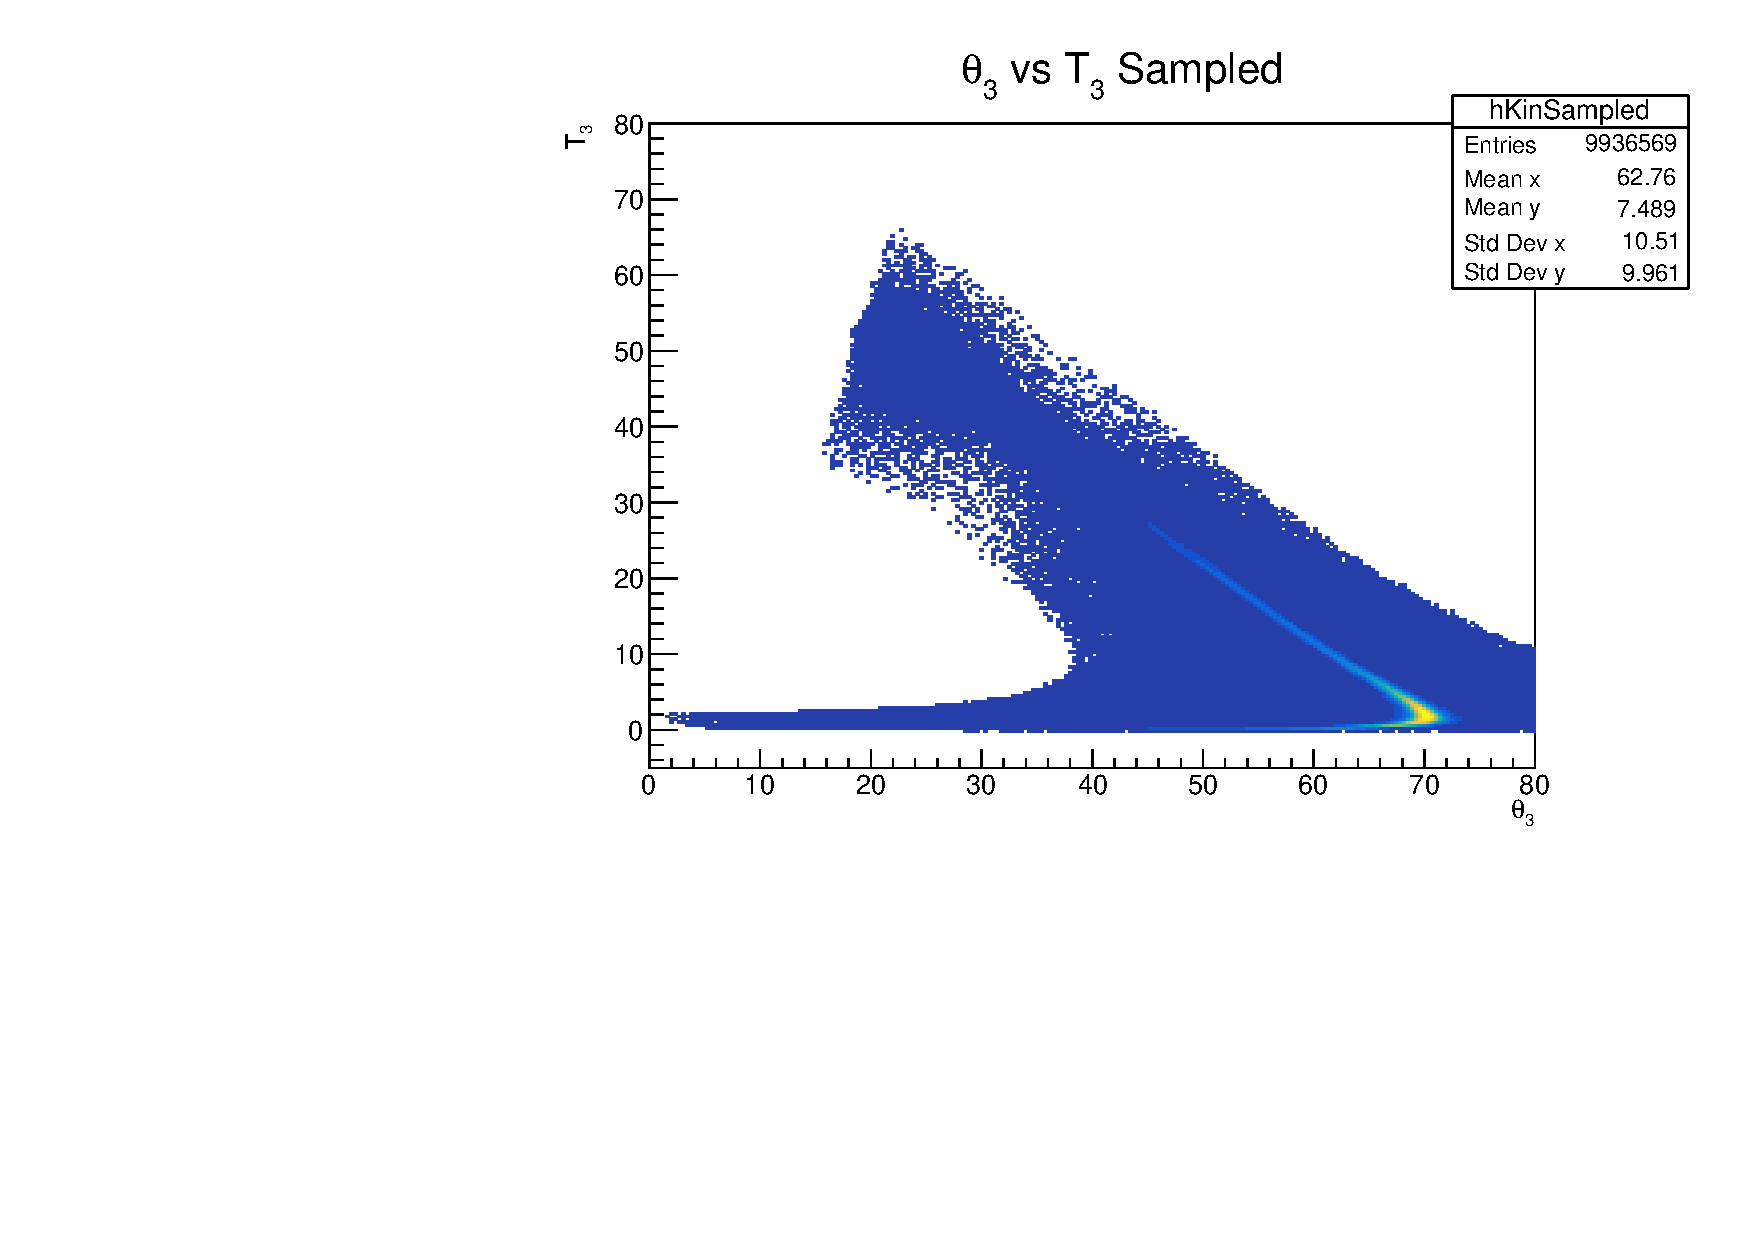
\includegraphics[width=1\linewidth]{Imagenes/KinSampled_Ex0.20_incIdx0.pdf}
        \captionof{figure}{Cinemática sampleada para $E^*=0.2$ MeV.}

        \label{Fig:04-kinSampled2}
    \end{minipage}

    \item También tendremos que tener en cuenta la distribución experimental de los ángulos $\theta_{cm}$, que tal y como ha sido descrito será una normal con FWHM de 1$^{\circ}$. Así pues, tendremos que aplicar esta distribución nada más obtener un $\theta_{cm}$. 

    
    \item Lo siguiente que debemos considerar es si la partícula llega a alguno de los silicios, ubicados según la geometría de \cref{Fig:Geo_Actar}. Para ello trazamos una recta con la dirección del tritio y calculamos la energía con la que llega a dicho silicio. Si la energía es mayor que cero y alcanza a uno de estos su detección es posible. Lógicamente deberemos considerar straggling y pérdidas de energía, por lo que gran parte de los tritios no llegarán a los silicios. Sin embargo esto no es un problema, ya que gracias a la TPC podremos recostuir la trayectoria de aquellos que se paren justo antes. En la \cref{Fig:04-Impacts} podemos ver la distribución de los tritios que llegan a los silicios, considerando todos los impactos y no solo los medidos. 
    
    Cuando una partícula llega con una energía suficientemente grande como para atravesar, la energía depositada será muy pequeña, ya que la ecuación de Bethe nos dice que la energía depositada es inversamente proporcional a la energía cinética de la partícula. Por tanto, si la partícula atraviesa el silicio no podremos reconstruir su trayectoria, y por tanto no podremos reconstruir la cinemática de la reacción. 

    \begin{center}
        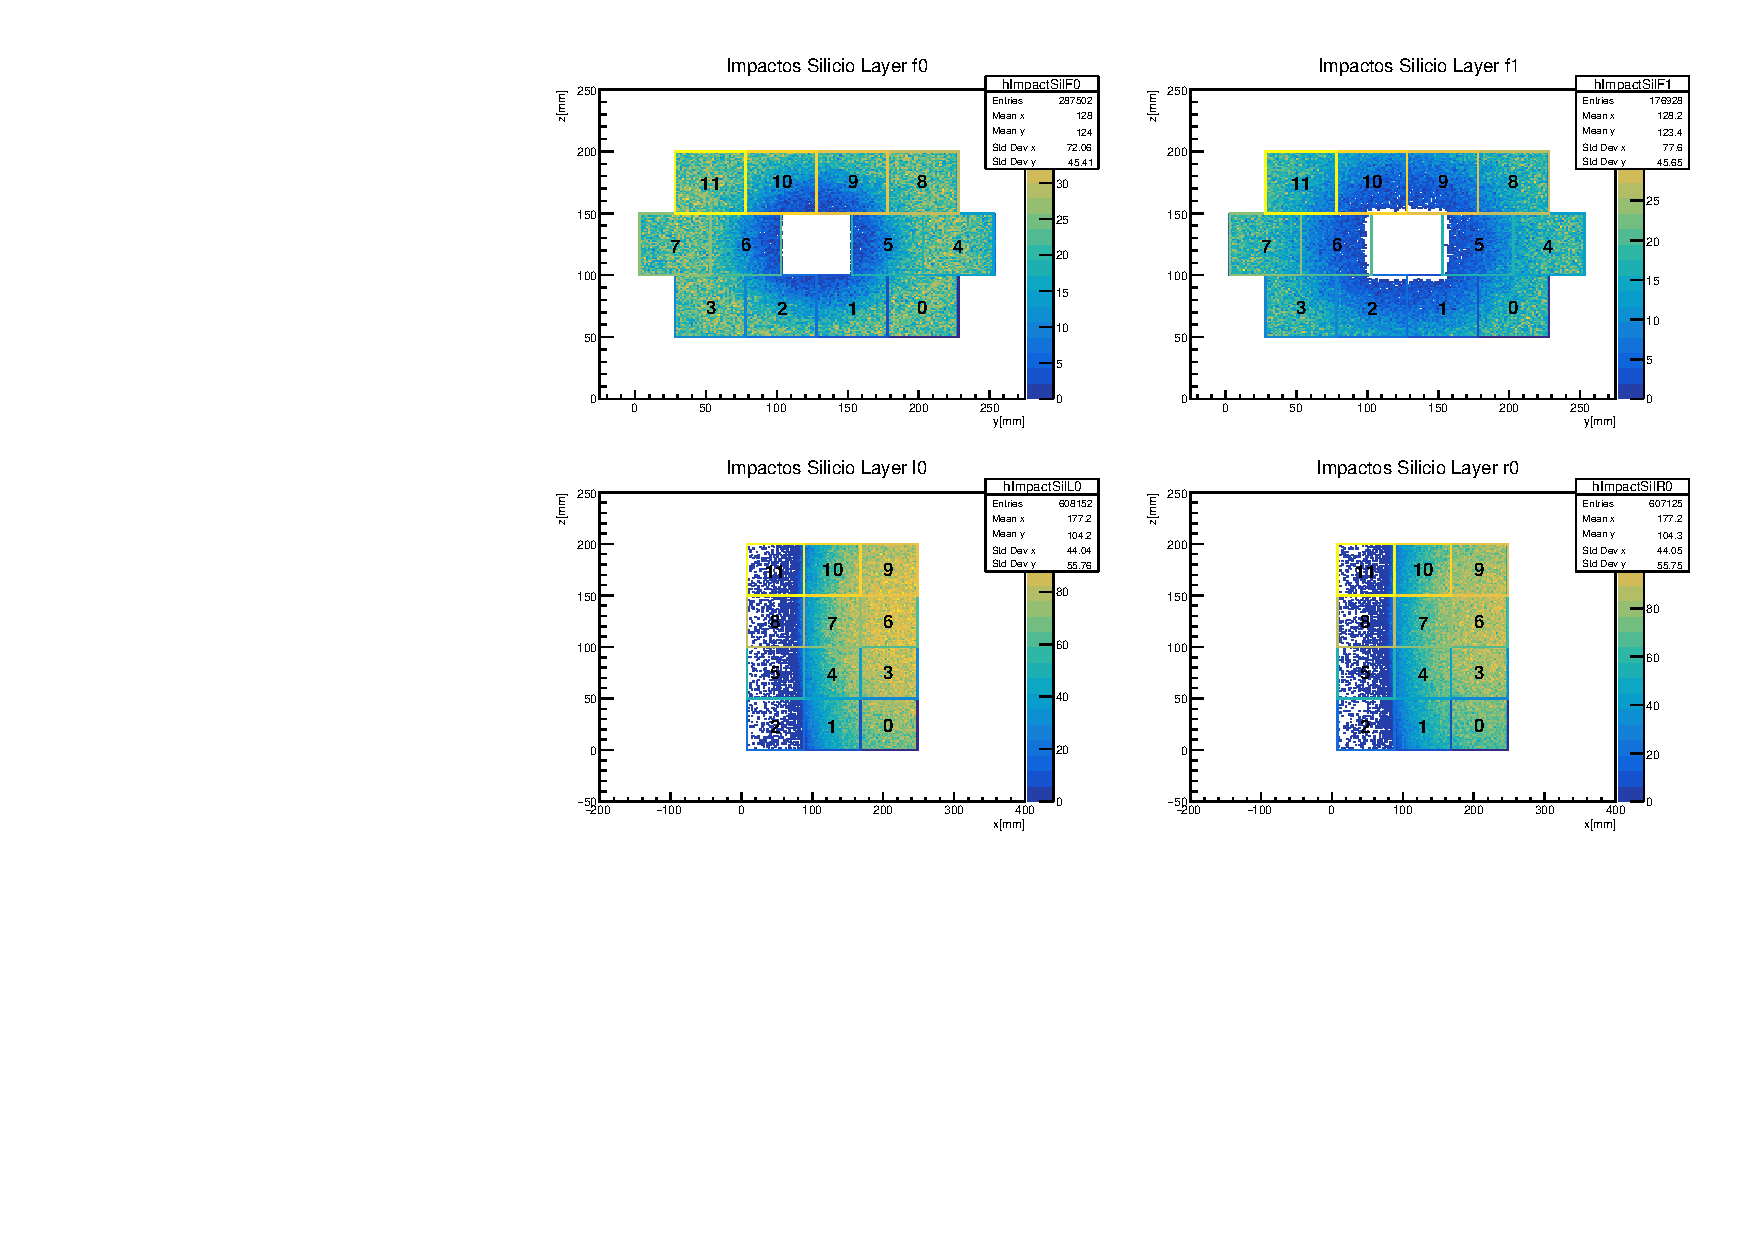
\includegraphics[width=0.8\linewidth]{Imagenes/Impacts_Ex0.00_incIdx0.pdf}
        \captionof{figure}{Distribución de los impactos en las 4 layers de silicios. }

        \label{Fig:04-Impacts}
    \end{center}
    

    Por tanto, con la disposición de Silicios actuales, no podremos detectar aquellos con ángulos de salida muy grandes, mientras que aquellos con un ángulo de salida muy pequeño no serán detectados bien porque se corresponden con una energía muy pequeña, y por tanto se frenan antes, o porque se corresponden con una energía muy grande y por tanto atraviesan los silicios sin detenarse. 

    Precisamente por esta razón se implementa en la cara contraria a la entrada de las partículas una capa de silicios doble, para poder ampliar el número de partículas detectadas y así poder obtener una mejor estadística. Para poder afirmar que una partícula ha sido detectada entonces tendrá que frenarse en alguno de los silicios l0, r0, f0 o f1. En aquellos que se frenen en f1 tendremos que considerar la enerǵia depositada también en el silicio f0 así como las energías pérdidas entre ambos silicios.

    La energía depositada real la obtendremos como una distribucción gaussiana centrada en la energía depositada promedio dada por la ecuación de Bethe y la $\sigma$ dada por la resolución dada por \label{Eq:Resolucion_Silicios}.

    \item A partir de las energías depositdas en los siliicios, y la posición en la que han sido detectados, podemos determinar unequívocamente la energía del tritio en el punto de interacción. Conociendo la energía cinética y en ángulo $\theta_{CM}$ podemos predecir unequívocamente la energía de excitación del $^{10}$Li, ya que esta determina la curva de la cinemática, tal y como podemos ver en la \cref{Fig:04-Kin}. Debido a los procesos estocásticos de péridda de energía y la incertidumbre del ángulo medido, la energía de excitación que podamos recostruir no será una Briet-Wigner, sino una convolución de la distribución de Breit-Wigner con una gaussiana, que nos dará una distribución de energía de excitación del $^{10}$Li. A partir de esta distrbución podremos obtener el valor de la energía de excitación, cual es el valor de $\sigma$ dada por todas las combinaciones y $\Gamma$. Lógicamente el valor medio de la energía de excitación y la anchura de la resonancia serán los valores que le hayamos introducido. Entre las diferentes combinaciones que encontramos tenemos:
    
    \begin{equation}
        \sigma_{tot}^2 = \sigma_{straggling}^2 + \sigma_{sil}^2 + \sigma_{\theta}^2 
    \end{equation}
    Seleccionando que incertidumbres queremos consdierar podremos evaluar que contribucción tiene cada una de ellas, y por tanto cual afecta más al experimento, al menos según el modelo aquí considerado. 

\end{enumerate}    
